\documentclass[Modultest/Modultest_main.tex]{subfiles}
\begin{document}

\lstdefinestyle{customc}{
    breaklines=true,
    language=C,
    showstringspaces=false,
}
\lstset{style=customc}

\section{WebPage Modultest}

Modulet WebPage har til opgave at modtage brugerinputs i form af brugernavne, holdnavne og holdfarver og sende disse til GameController klassen. Herfra skal de videreformidles til resten af systemet, herunder playersides og display. Det er imidlertid vigtigt at WebPage sender de rigtige informationer, og at der sjældent sker fejl i afsendingen. \\\\WebPage er svær at teste isoleret, da den baserer sig på kommunikation med GameController klassen og er afhængig af denne. For at teste hjemmesiden og sikre, at kravene er opfyldt, er der derfor udviklet et separat program til formålet. Denne test stub skal simulere GameController klassen, så det kan undersøges, om den modtager de rigtige informationer, når de sendes fra hjemmesiden. Der implementeres en C++ klasse kaldet WebPage og en C++ klasse kaldet GameController. Der anvendes den event drevne arkitektur, som er beskrevet i afsnittet "Design af RPiApp - USER SPACE". Det betyder at programmet anvender messages og message queues, samt klasserne Thread og ThreadFunctor til at håndtere tråde. I main oprettes GameControllers MsgQueue samt to tråde, hhv. WebPageThread og GameThread. Dette er vist i kodeeksemplet nedenfor.
\begin{lstlisting}
int main()
{
    MsgQueue GameControllerMsgQueue_;
    GameController GameControllerObj_(&GameControllerMsgQueue_);
    WebPage WebPageObj_(&GameControllerMsgQueue_);

    Thread GameThread(&GameControllerObj_);
    Thread WebPageThread(&WebPageObj_);

    GameThread.start();
    WebPageThread.start();
	
    GameThread.join();
    WebPageThread.join();
}
\end{lstlisting}
WebPageThread lytter på port 3000, og når der genereres et event fra client, dvs. der trykkes start på hjemmesiden sendes informationerne i form af en besked kaldet WebPageRespone til GameController. Når denne modtager beskeden sørger dispatcher systemet for at switche ud på beskedens ID. I dette tilfælde bliver informationerne for hold 1 og hold 2 udskrevet i terminalen, så det kan bekræftes, at kommunikationen forløber korrekt, og at data er som forventet. Dele af dispatcheren og handleren fremgår nedenfor.
\begin{lstlisting}
void GameController::dispatcher(unsigned long messageID, Message * msg)
{
    switch (messageID) 
    {
        case ID_INFO_READY:
	    {
	WebPageResponse * ind = static_cast<WebPageResponse *>(msg);

	std::cout << "Team 1:" << std::endl;
	std::cout << "Teamname is: " << ind->team1_.getTeam() << std::endl;
	std::cout << "Username1 is: " << ind->team1_.getUser1() << std::endl;
	std::cout << "Username2 is: " << ind->team1_.getUser2() << std::endl;
	std::cout << "Red is: " << ind->team1_.getRed() << std::endl;
	std::cout << "Green is: " << ind->team1_.getGreen() << std::endl;
	std::cout << "Blue is: " << ind->team1_.getBlue() << std::endl << std::endl;

	std::cout << "Team 2:" << std::endl;
	...
    	}
    }
}
\end{lstlisting}

Figur \ref{fig:WebPage_1} viser hjemmesidens interface i browseren og resultatet af testen er vist med et terminal output i figur \ref{fig:WebPage_2}. Det fremgår at holdnavne, brugernavne og holdfarver er sat som forventet. I ikke-funktionelle krav for WebPage er det specificeret i krav K5.8, at der højst må ske en fejl i afsendingen 1 ud af 20 gange. Derfor gentages ovenstående test nu x antal gange, mens navne og farver varieres. Resultatet fremgår af tabel x. Konfidensniveauer.

\begin{figure}[H]
    \centering
    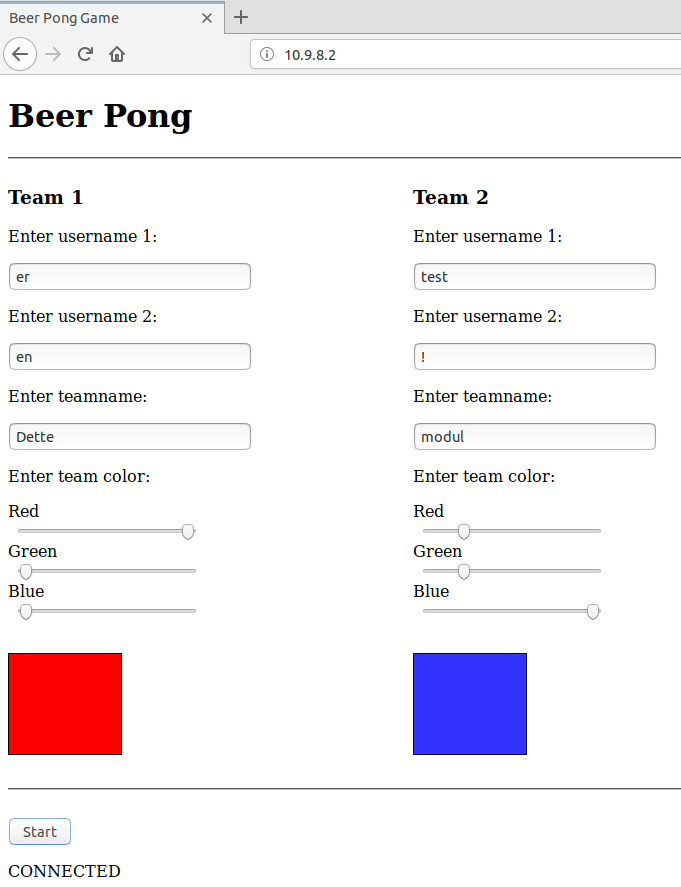
\includegraphics[width=0.9\textwidth]{Modultest/WebPage/graphics/modultest_1.png}
    \caption{Modultest af WebPage - hjemmeside vist i browser}
    \label{fig:WebPage_1}
\end{figure}
\begin{figure}[H]
    \centering
    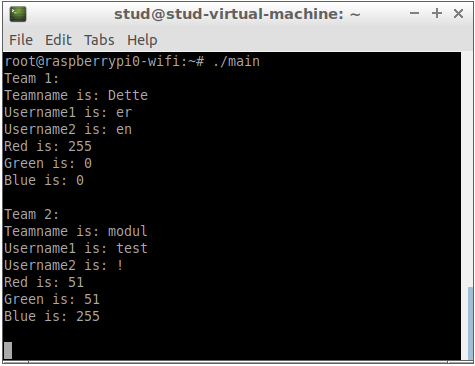
\includegraphics[width=\textwidth]{Modultest/WebPage/graphics/modultest_2.png}
    \caption{Modultest af WebPage - output vist i terminal}
    \label{fig:WebPage_2}
\end{figure}

\end{document}